\documentclass{beamer}
\usepackage{graphicx}
\usepackage{amsmath}
\usepackage{amsfonts}
\usepackage{amssymb}
\usepackage{pdfpages}
\usepackage[all]{xy}
\usetheme{AISEC}
\setbeamercovered{transparent}

% Load Fraunhofer font
\IfFileExists{fhgfon.tsty}
{
    \usepackage{fhgfont}
}
{
    % Font Settings: rev. Times, rev. Helvetica and DejaVuSansMono
    \usepackage[notext]{stix}
    \usepackage{tgtermes}
    \usepackage[scale=0.92]{tgheros}
    \usepackage[scaled=0.80]{DejaVuSansMono}
}

% Better typography
\usepackage[
    activate={true,nocompatibility},
    final,
    tracking=true,
    kerning=true,
    spacing=true,
    babel=true,
]{microtype}

% Codelistings
% \usepackage[]{minted}
% \usemintedstyle{bw}

% Configure linenumbers of code blocks
% \renewcommand{\theFancyVerbLine}{
%     \sffamily
%     \textcolor{black}{\scriptsize\arabic{FancyVerbLine}}
% }
%
% Example for a minted python environment:
% \newminted{python}{
%     fontsize=\normalsize,
%     numbersep=10pt,
%     xleftmargin=1pt,
%     xrightmargin=1pt
% }

% Load and set up input encoding and babel
\usepackage[utf8]{inputenc}
\usepackage[english]{babel}

% Load and set up other packages
%\graphicspath{{./figures/}} % Set the search path for graphics


% Configure Fraunhofer beamer theme

% Disable the infoline in the footer [default: enabled]
% \infolinefalse

% Enable automatic numbering of frame titles and subtitles;
% used in conjunction with sectioning [default: disabled]
% \numberingtrue

% Disable the use of squares in itemize environments [default: enabled]
% \usesquaresfalse

% Disable the extended title page headline [default: enabled]
% \extendedtitlefalse

% Display  red CONFIDENTIAL string in the infoline [default: disabled]
% \confidentialtrue


% Set title page infromation
\title[Short Title]{Post-quantum secure PUF authentication using LPN}
\subtitle[Short Subtitle]{ }
\author[Short Author]{Han Zhao}
\date{\today}


% Set contact page information
\name{\insertauthor}
\department{Group Product Protection\newline Department Security and Trusted OS}
\institute{Fraunhofer-Institute for\newline Applied and Integrated Security (AISEC)}
\address{Parkring 4\newline 85748 Garching (near Munich)\newline Germany}
\web{http://www.aisec.fraunhofer.de}
\phone{+49 16 25231418}
\fax{+49 89 3229986-222}
\email{ga84fif@mytum.de}


\begin{document}

\begin{titleframe}
    \titlepage
    \vskip2.7cm
    \begin{center}
        
\includegraphics[scale=.7]{aisec_logo.pdf}
    \end{center}
\end{titleframe}

\begin{outlineframe}
%    \frametitle{Outline}
    \tableofcontents
\end{outlineframe}

% Content
\section{Introduction}

\begin{outlineframe}
	\tableofcontents[currentsection]
\end{outlineframe}
\subsection{Concept}
\begin{frame}
	\alert{LPN}:  Learning Parity with Noise \\
	\vspace{0.2cm}
	\begin{description}
		\item[1.] Randomly select a secret \alert{s} in GF(2)
		\item[2.] Randomly select \alert{A} from GF(2)
		\item[3.] Select a bit offset \alert{e} $\longrightarrow$ $Ber_{\epsilon}$
		\item[4.] Output \alert{b}= $<$ A*s+e $>$ as a sample\\
		\vspace{0.4cm}
		\alert{	\Large{	$b_{i} = A_{i}$*$s+e_{i}$ ~~~~mod~~2~~~~with i={0,1,...,m}}}\\
	\end{description}
	\vspace{0.2cm}
			\vspace{0.5cm}		
	The goal: \\
	\vspace{0.2cm}
	\centering
	Find s given only the values of b and A.\\ 
\end{frame}





\subsection{Motivation}
\begin{frame}
	\begin{itemize}
		\item Fundamental in theory for LPN%strong PUF VS weak PUF
		\begin{itemize}
			\item Equivalent to decoding random linear codes
			\item Believed to be hard%: no polynomial time algorithm is known.
		\end{itemize}	
	\end{itemize}

\end{frame}


\begin{frame}
	\frametitle{Motivation}
	\framesubtitle{LPN -- Problem}
	 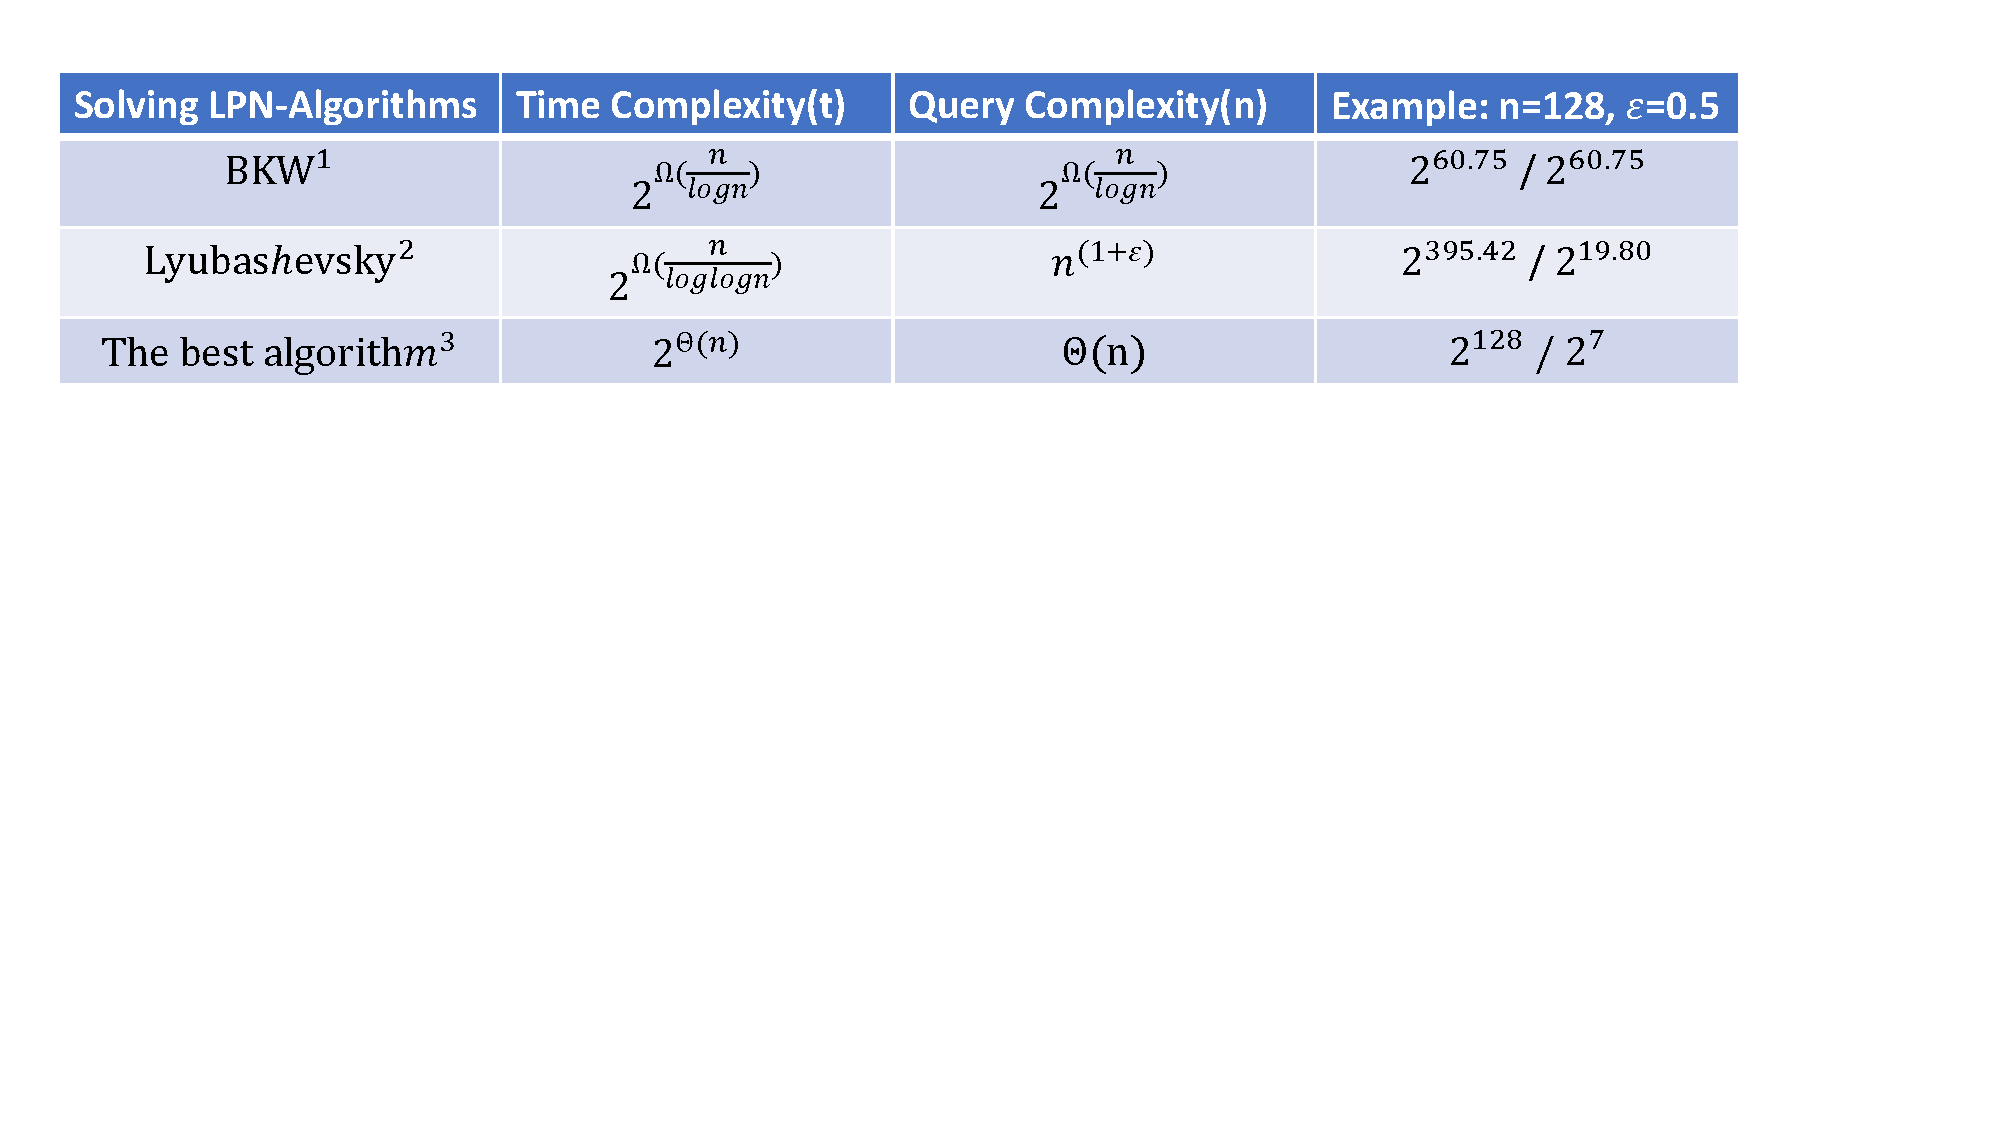
\includegraphics[width=5.2in,height=4.8in]{LPN-algorithm.pdf}
	\vspace{0.5cm}
\end{frame}


%\subsection{Motivation}
\begin{frame}
	\begin{itemize}
		\item Many applications in Cryptographic %% LPN -- NP Problem
		\begin{itemize}
			\item User authentication, encryption, etc
			\item Cryptographic primitives%Traditional Encryption VS One-time-pad
		\end{itemize}
	\end{itemize}
\vspace{0.5cm}
\begin{columns}[c]
	\column{6cm}
	
		Strong PUF-authentication:
		\begin{itemize}
			\item [---] information-theoretical complexity
			\item [---] no protection mechanisms
			\item [---]	not post-processed on chip
		\end{itemize}
	\column{6cm}
		LPN-authentication:
		\begin{itemize}
		\item [---] computational complexity
		\item [---] no known quantum-attacks 
		\item [---]	post-quantum cryptography
		\end{itemize}		
\end{columns}
	%	\begin{itemize}
	%		\item Traditional Encryption VS One-time-pad
	%	\end{itemize}
	%	\vspace{0.2cm}
	
\end{frame}


%\subsection{Notation}
%\begin{frame}
%	\alert{TRNG}: True Random Number Generator\\
%	\vspace{0.2cm}
%	\alert{A}: publicly known matrix (Generator Matrix)\\
%	\vspace{0.2cm}
%	\alert{e}: the initial reference response of PUF\\
%	\vspace{0.2cm}
%	\alert{e{'}}: the PUF response of the identical challenge in later time\\
%\end{frame}



\section{The construction of the authentication system}
\begin{outlineframe}
	\tableofcontents[currentsection]
\end{outlineframe}


\subsection{Enrollment phase}
\begin{frame}
    \frametitle{The construction of the authentication system}
    \framesubtitle{Enrollment phase}
%    \begin{alertenv}
%    	Reference challenge-response pairs are collected:
%    \end{alertenv}
    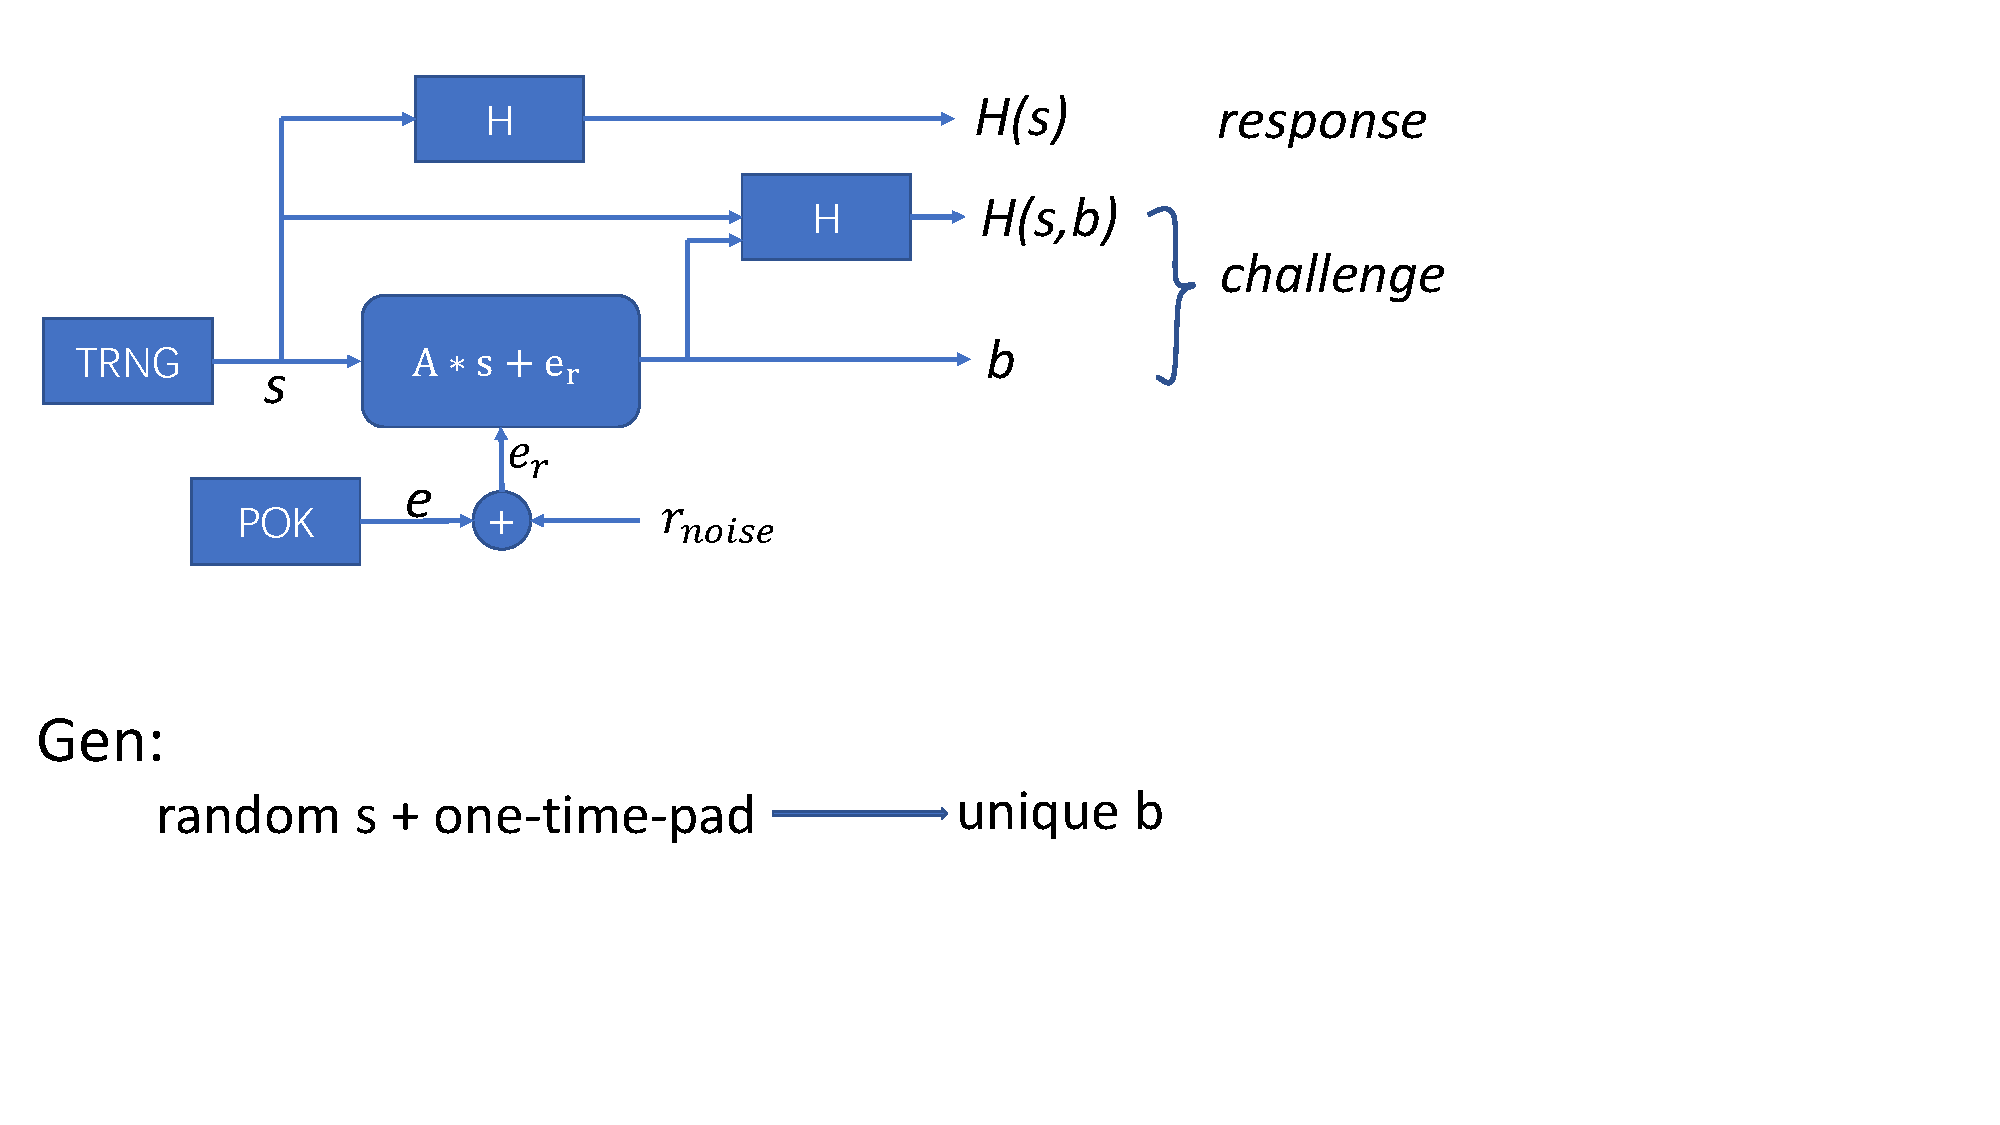
\includegraphics[width=5in,height=3in]{Enrollment-phase.pdf}
\end{frame}


\subsection{Authentication phase}
\begin{frame}
	\frametitle{The construction of the authentication system}
	\framesubtitle{Authentication phase}
	\vspace{0.5cm}
	\centering
	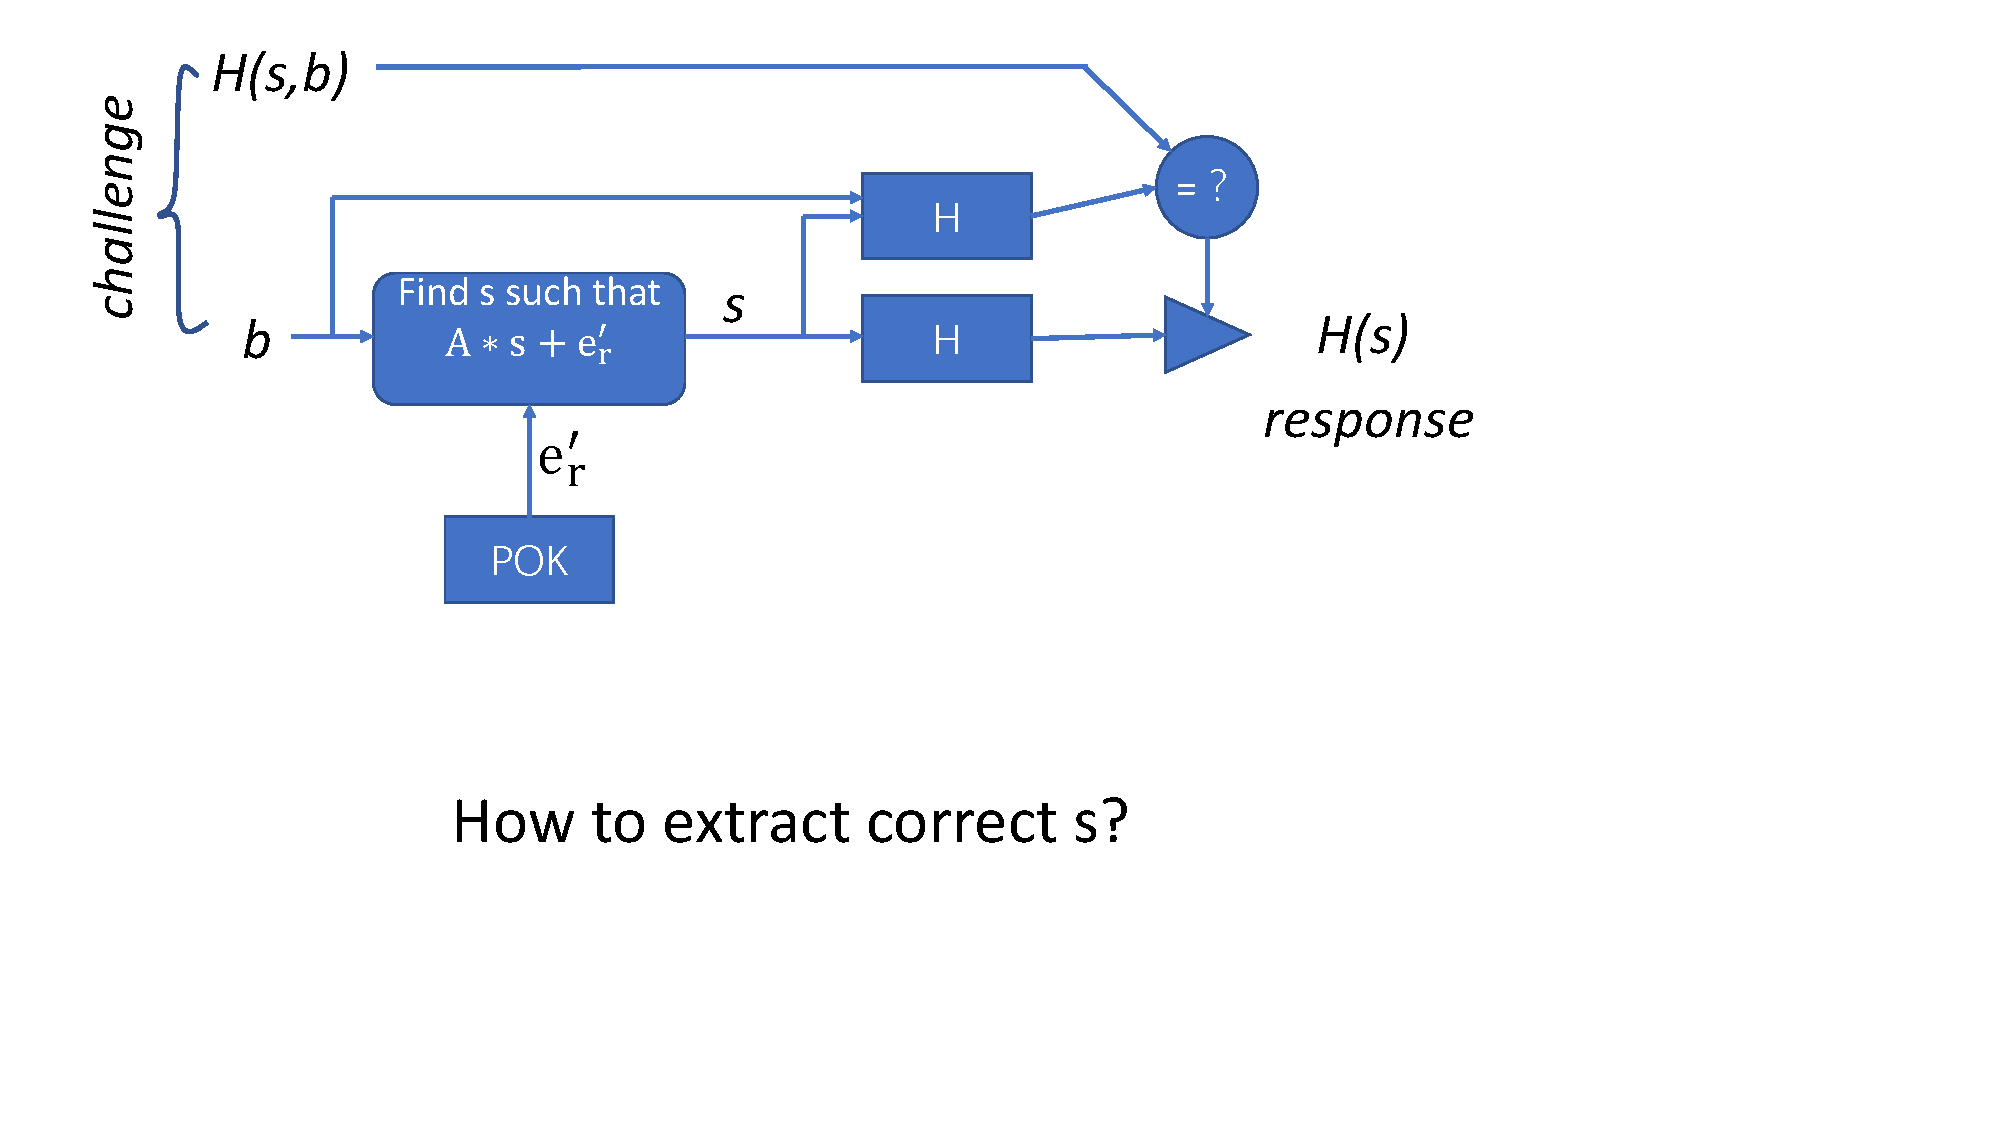
\includegraphics[width=5in,height=3in]{Authentication-phase.pdf}\\
\end{frame}


\begin{frame}
	\frametitle{The construction of the authentication system}
	\framesubtitle{Authentication phase}
	{\Large	Extracting s in the decoding module:}\\
	\vspace{0.5cm}
	\begin{itemize}
		\item Gaussian elimination algorithm 	
		\begin{itemize}
			\item [---] suitable for linear equations
			\item [---] complex implementation in hardware
		\end{itemize}
	
	\end{itemize}
	\begin{itemize}
		\item Error correction algorithm
		\begin{itemize}
			\item [---] accurate extraction 
			\item [---] no security reduction
		\end{itemize}
	\end{itemize}
\end{frame}



\begin{frame}
	\frametitle{Authentication phase}
	\framesubtitle{Error correction codes}
	\begin{columns}
		\begin{column}{0.52\textwidth}
			LDPC Code\\
			\begin{itemize}
				\item complex construction of PC matrix\\
			\end{itemize}
			\begin{itemize}
				\item complex encoding module\\
			\end{itemize}
			\begin{itemize}
				\item suitable for long code
			\end{itemize}		
		\end{column}
		\begin{column}{0.48\textwidth}
			Reed-Muller Code\\
			\begin{itemize}
				\item the simple construction\\
			\end{itemize}
			\begin{itemize}
			\item no parity check matrix\\
			\end{itemize}
			\begin{itemize}
				\item good error correction property
			\end{itemize}			
		\end{column}
	\end{columns}
\end{frame}


\begin{frame}
	\frametitle{Reed Muller Code}
	\framesubtitle{The Plotkin-Construction^{4}}
%	Characterization of RM(r,m) codes with the parameters r and m:\\
%	\vspace{0.2cm}
%	$n=2^{m}$	\\
%	\vspace{0.2cm}
%	$k=\sum_{i=1}^r $$\left(\begin{aligned} m\\i \end{aligned} \right) $   \\
%	\vspace{0.2cm}
%	$ d = {2^{m \textnormal{-} r}} $ \\

Plotkin construction with two subcodes for RM(r,m):\\
	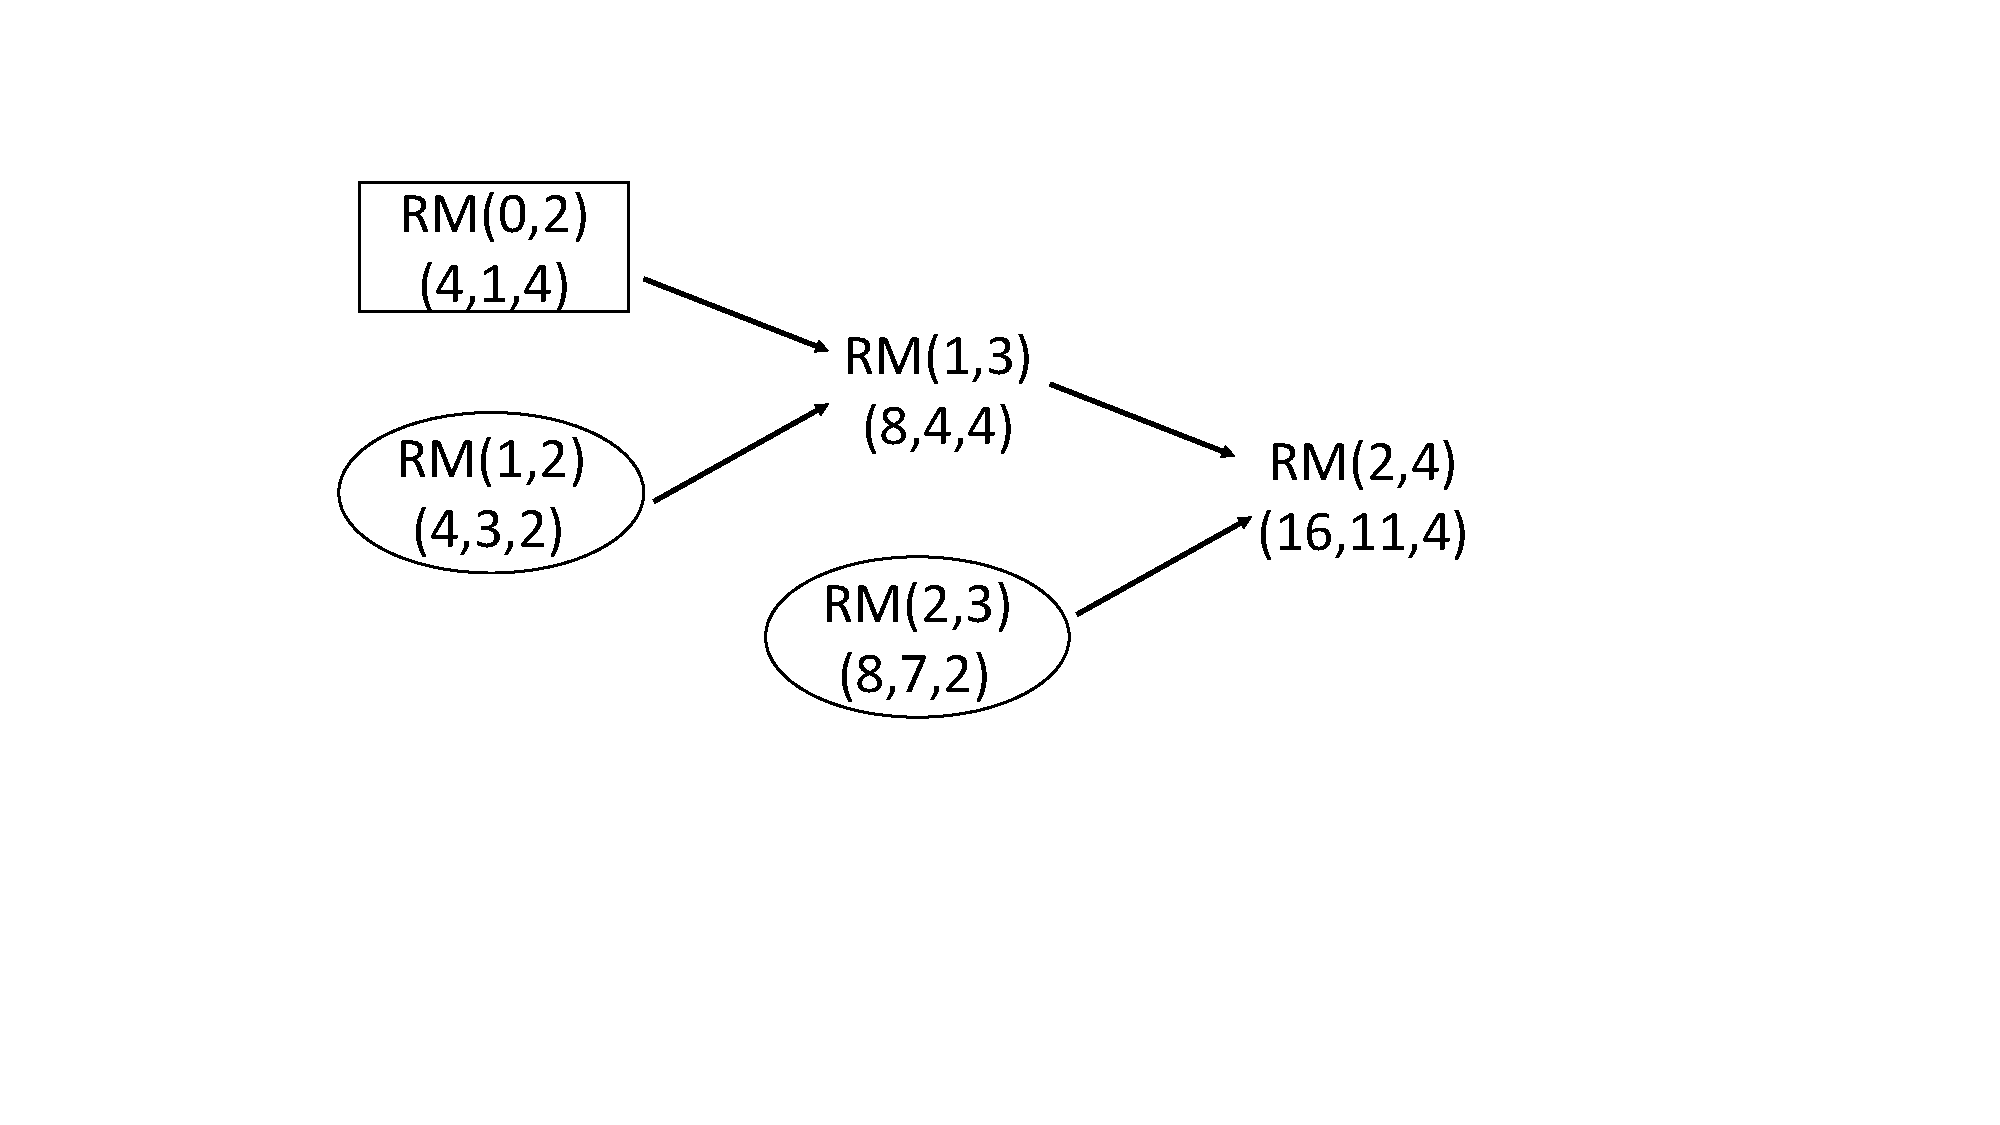
\includegraphics[width=4.8in,height=2.3in]{PlotkinRM24.pdf}\\
	\large{c = ( $ u \left|  u + v \right$ )	 $:$	u  $\epsilon$ RM(r,m{-}1), v $\epsilon$ RM(r{-}1,m{-}1)}\\
	\vspace{0.5cm}
\end{frame}




\begin{frame}
	\frametitle{Decoding Algorithm}
	\framesubtitle{GMC algorithm VS Recursive algorithm}
	\begin{columns}
		\begin{column}{.48\textwidth}
			\alert{GMC Algorithm:}\\
			\vspace{0.5cm}
			analysis for AWGN-channel\\
			\vspace{0.2cm}
			complex to realise in hardware\\
		\end{column}
		\begin{column}{.48\textwidth}
			\alert{Recursive Algorithm:}\\
			\vspace{0.5cm}
			analysis for BEC\\
			\vspace{0.2cm}
			easy to operate in hardware
		\end{column}
	\end{columns}
\end{frame}


\begin{frame}
	\frametitle{Reed Muller Code}
	\framesubtitle{The Recursive Decoding Algorithm^{4}}
	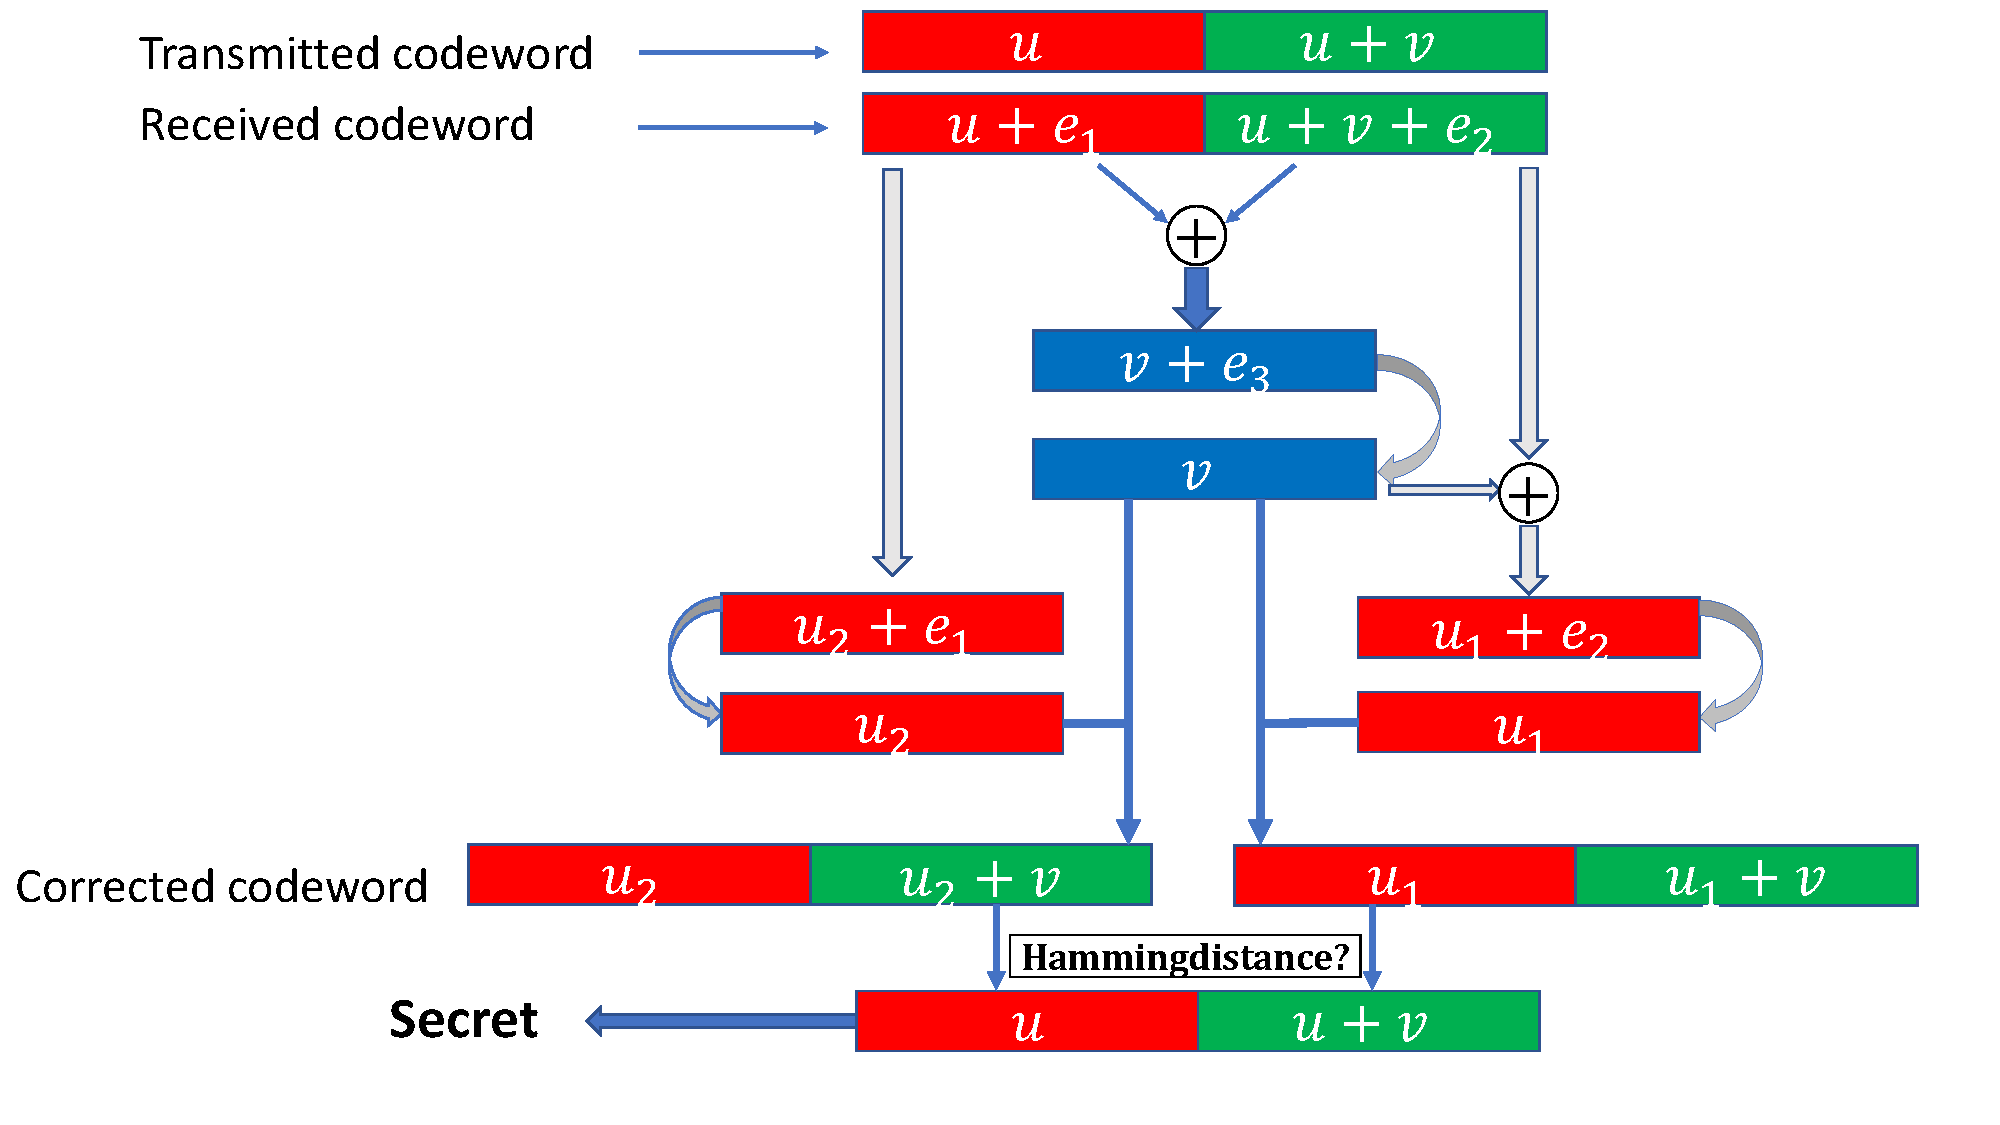
\includegraphics[width=5in,height=3in]{recursivedecoding-description.pdf}
\vspace{0.5cm}
\end{frame}


\section{Conclusion}
\begin{outlineframe}
	\tableofcontents[currentsection]
\end{outlineframe}
\begin{frame}
	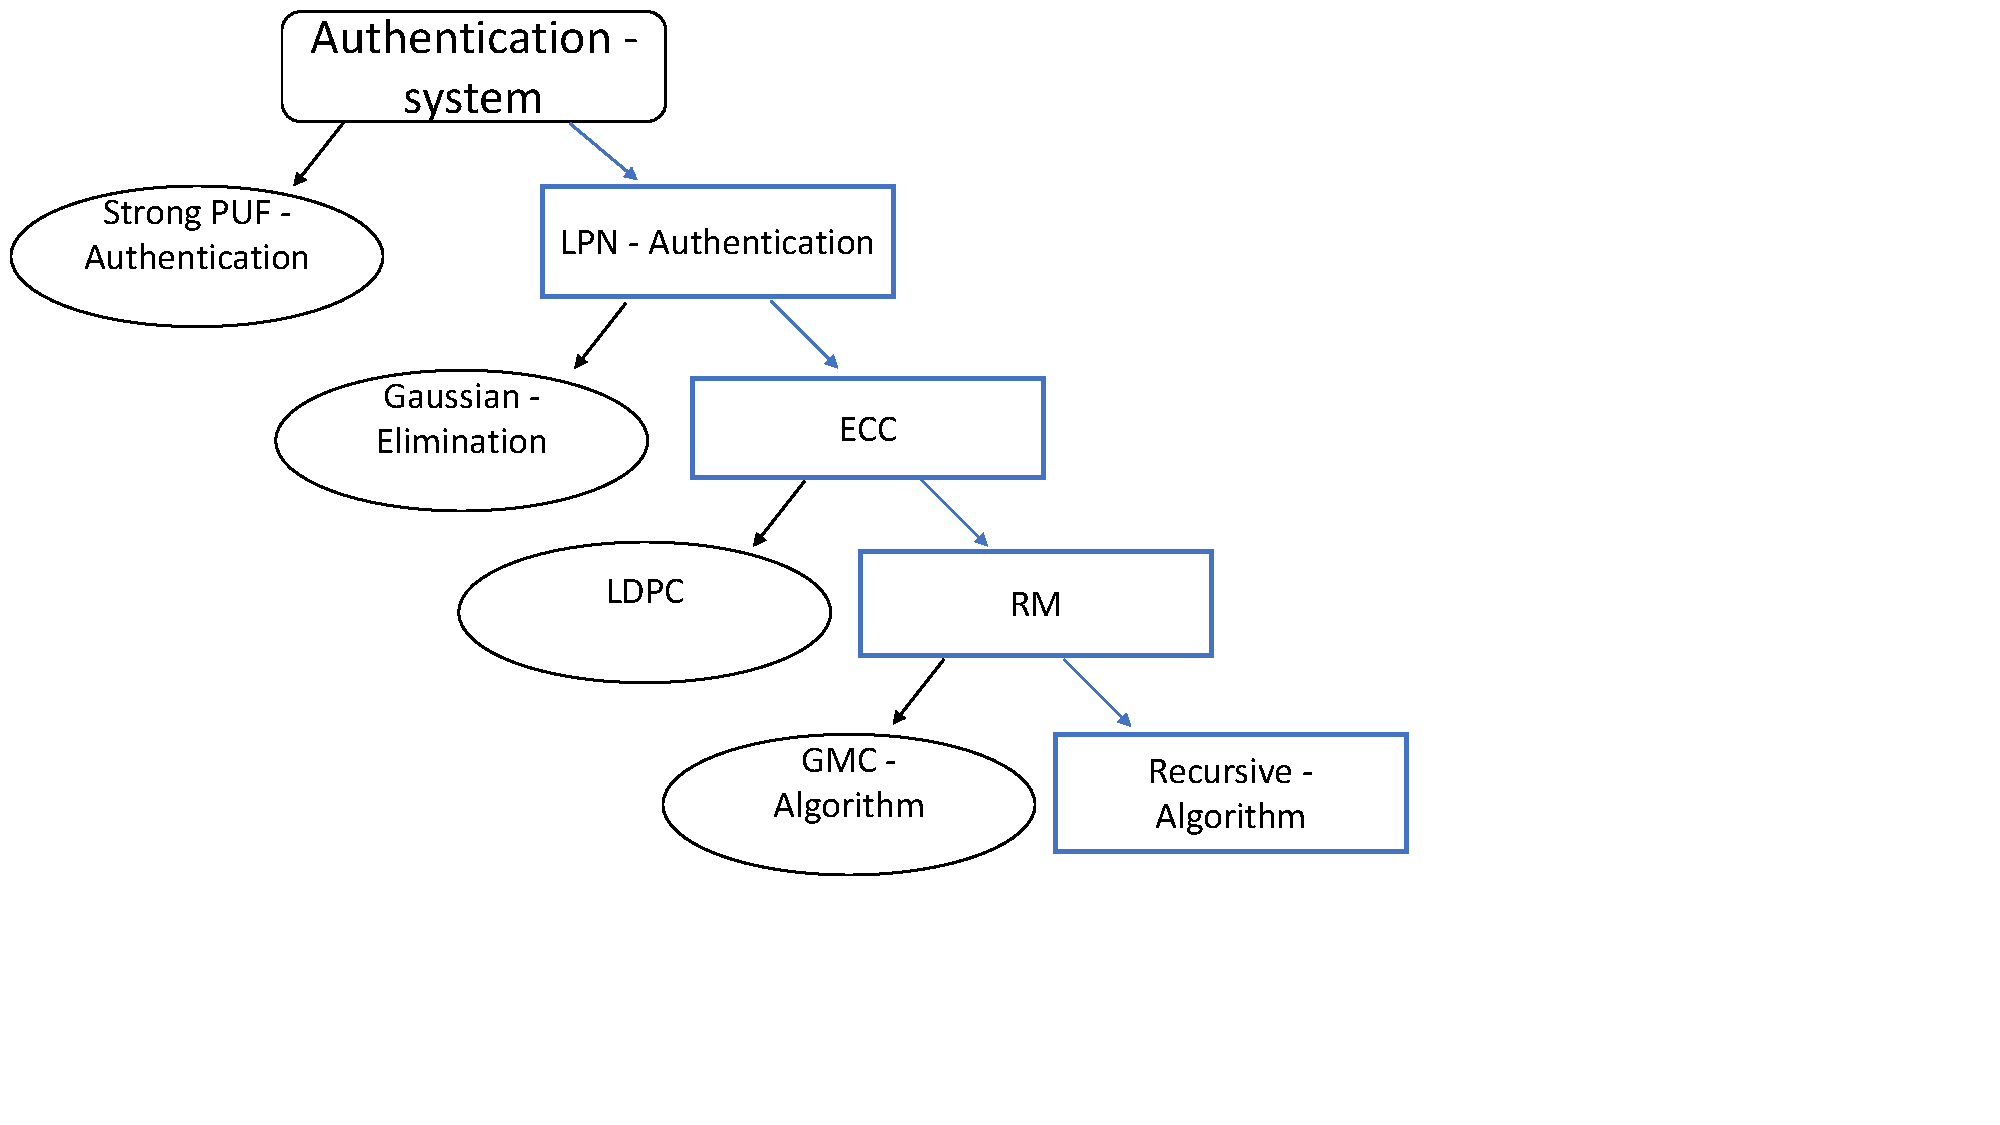
\includegraphics[width=6.2in,height=3.5in]{conclusion.pdf}
\end{frame}	


\section{Schedule}
\begin{outlineframe}
	\tableofcontents[currentsection]
\end{outlineframe}
\begin{frame}
	\vspace{0.3cm}
	\centering
	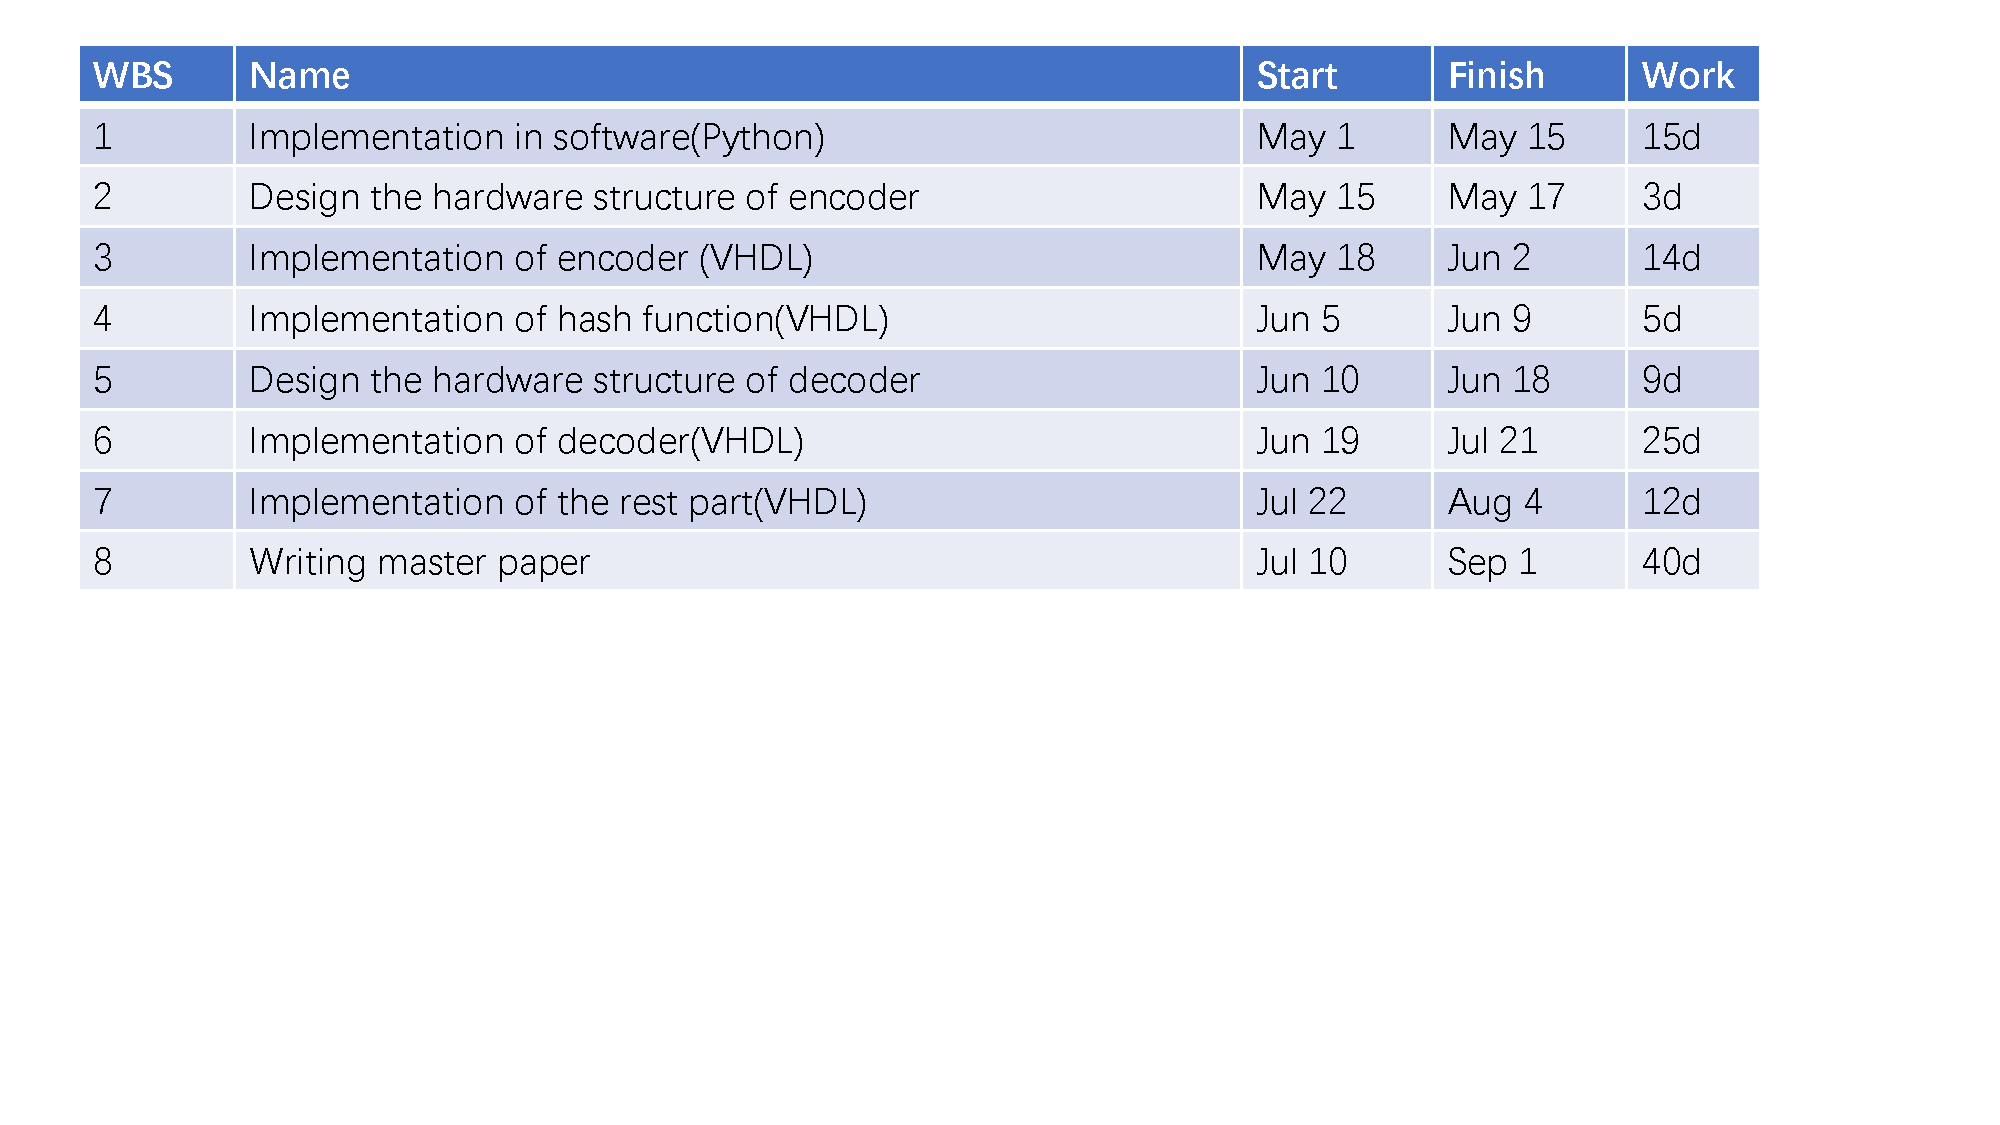
\includegraphics[width=5in,height=3.8in]{Schedule.pdf}
\end{frame}	



\section{Bibliography}
\begin{outlineframe}
	\tableofcontents[currentsection]
\end{outlineframe}
\begin{bibliographyframe}
	{\leftskip=0pt \rightskip=0pt plus 0cm
	\small{
$[1]$ A. Blum, A. Kalai, and H. Wasserman, “Noise-tolerant learning, the parity problem, and the statistical query model,” J. ACM, vol. 50, no. 4, pp. 506–519, 2003.\\
$[2]$ V. Lyubashevsky, “The parity problem in the presence of noise, decoding random linear codes, and the subset sum problem,” in Proc. 8th Int. Workshop Approximation, Randomization Combinatorial Optimization Algorithms Techn., 2005, pp. 378–389.\\
$[3]$ Qian Guo, Thomas Johansson, and Carl L¨ondahl. Solving LPN Using Covering Codes. In Palash Sarkar and Tetsu Iwata, editors, Advances in Cryptology - ASIACRYPT 2014 - 20th International Conference on the Theory and Application of Cryptology and Information Security, Kaoshiung, Taiwan, R.O.C., December 7-11, 2014. Proceedings, Part I, volume 8873 of Lecture Notes in Computer Science, pages 1–20. Springer, 2014.\\
$[4]$ Bossert, Martin: Kanalcodierung. 3., überarb. Aufl. München : Oldenbourg, 2013. – XVIII, 531 S. : graph. Darst.. – ISBN 978–3–486–72128–7 – 978–3–486–75516–9 \\
}
}
\end{bibliographyframe}

\section{Discussion}
\begin{outlineframe}
	\tableofcontents[currentsection]
\end{outlineframe}
\begin{frame}
	\frametitle{Discussion}
	\center{{\Large Question? }}\\	
\end{frame}	

\begin{frame}
	\frametitle{Post-quantum cryptography}
	Post-quantum cryptography: \\
	\begin{itemize}
		\item refers to cryptographic algorithms (usually public-key algorithms)\\ 
	\end{itemize}
	\begin{itemize}
		\item secure against an attack by a quantum computer.\\
	\end{itemize}
	\begin{itemize}
	\item distinct from quantum cryptography, which uses quantum phenomena to achieve secrecy and detect eavesdropping\\ 
	\end{itemize}
\end{frame}	


\begin{frame}
	\frametitle{Weak PUF vs Strong PUF}
		\begin{columns}
			\begin{column}{.48\textwidth}
				\alert{Weak PUF:}\\
				\vspace{0.3cm}
				key generation\\
				input and output with same length\\ 
				a small number of CRPs\\
				\vspace{0.5cm}
			\end{column}
			\begin{column}{.48\textwidth}
				\alert{Strong PUF:}\\
				\vspace{0.3cm}
				authentication protocol\\
				long input, short output\\
				large enough CRP space\\
				\vspace{0.5cm}
			\end{column}
		\end{columns}
\end{frame}

\begin{frame}
	\frametitle{Security parameter}
	for this system a key size of n :\\
	\vspace{0,5cm}
	\begin{itemize}
		\item each of the 3 famous algorithms performs worse than brute-force or does not succeed at all^{5}.\\ 
	\end{itemize}
	\begin{itemize}
		\item for a security parameter of k= 128 against the best known attacks.\\
	\end{itemize}
%	When calculate the subcode of RM-Code, the information-bits s can also be calculated;\\
%	the analysis of decoding complexity of RM-Code\\	
\end{frame}	

\begin{frame}
	\frametitle{Parameter setting}
	for this system a key size of n :\\
	\vspace{0,5cm}
	\begin{itemize}
		\item Plan\quad A: \quad 2 * RM(3,7) \qquad (128,64,16)\\ 
	\end{itemize}
	\begin{itemize}
		\item Plan\quad B: \quad 1 * RM(3,9) \qquad (512,130,64)\\
	\end{itemize}
\end{frame}	



\begin{contactframe}
    \contactpage
\end{contactframe}

\end{document}